%% BioMed_Central_Tex_Template_v1.05
%%                                      %
%  bmc_article.tex            ver: 1.05 %
%                                       %


%%%%%%%%%%%%%%%%%%%%%%%%%%%%%%%%%%%%%%%%%
%%                                     %%
%%  LaTeX template for BioMed Central  %%
%%     journal article submissions     %%
%%                                     %%
%%         <27 January 2006>           %%
%%                                     %%
%%                                     %%
%% Uses:                               %%
%% cite.sty, url.sty, bmc_article.cls  %%
%% ifthen.sty. multicol.sty		       %%
%%									   %%
%%                                     %%
%%%%%%%%%%%%%%%%%%%%%%%%%%%%%%%%%%%%%%%%%


%%%%%%%%%%%%%%%%%%%%%%%%%%%%%%%%%%%%%%%%%%%%%%%%%%%%%%%%%%%%%%%%%%%%%
%%                                                                 %%	
%% For instructions on how to fill out this Tex template           %%
%% document please refer to Readme.pdf and the instructions for    %%
%% authors page on the biomed central website                      %%
%% http://www.biomedcentral.com/info/authors/                      %%
%%                                                                 %%
%% Please do not use \input{...} to include other tex files.       %%
%% Submit your LaTeX manuscript as one .tex document.              %%
%%                                                                 %%
%% All additional figures and files should be attached             %%
%% separately and not embedded in the \TeX\ document itself.       %%
%%                                                                 %%
%% BioMed Central currently use the MikTex distribution of         %%
%% TeX for Windows) of TeX and LaTeX.  This is available from      %%
%% http://www.miktex.org                                           %%
%%                                                                 %%
%%%%%%%%%%%%%%%%%%%%%%%%%%%%%%%%%%%%%%%%%%%%%%%%%%%%%%%%%%%%%%%%%%%%%


\NeedsTeXFormat{LaTeX2e}[1995/12/01]
\documentclass[10pt]{bmc_article}    



% Load packages
\usepackage{cite} % Make references as [1-4], not [1,2,3,4]
\usepackage{url}  % Formatting web addresses  
\usepackage{ifthen}  % Conditional 
\usepackage{multicol}   %Columns
\usepackage[utf8]{inputenc} %unicode support
%\usepackage[applemac]{inputenc} %applemac support if unicode package fails
%\usepackage[latin1]{inputenc} %UNIX support if unicode package fails
\urlstyle{rm}
 
 
%%%%%%%%%%%%%%%%%%%%%%%%%%%%%%%%%%%%%%%%%%%%%%%%%	
%%                                             %%
%%  If you wish to display your graphics for   %%
%%  your own use using includegraphic or       %%
%%  includegraphics, then comment out the      %%
%%  following two lines of code.               %%   
%%  NB: These line *must* be included when     %%
%%  submitting to BMC.                         %% 
%%  All figure files must be submitted as      %%
%%  separate graphics through the BMC          %%
%%  submission process, not included in the    %% 
%%  submitted article.                         %% 
%%                                             %%
%%%%%%%%%%%%%%%%%%%%%%%%%%%%%%%%%%%%%%%%%%%%%%%%%                     


\usepackage{graphicx}
%\def\includegraphic{}
%\def\includegraphics{}



\setlength{\topmargin}{0.0cm}
\setlength{\textheight}{21.5cm}
\setlength{\oddsidemargin}{0cm} 
\setlength{\textwidth}{16.5cm}
\setlength{\columnsep}{0.6cm}

\newboolean{publ}

%%%%%%%%%%%%%%%%%%%%%%%%%%%%%%%%%%%%%%%%%%%%%%%%%%
%%                                              %%
%% You may change the following style settings  %%
%% Should you wish to format your article       %%
%% in a publication style for printing out and  %%
%% sharing with colleagues, but ensure that     %%
%% before submitting to BMC that the style is   %%
%% returned to the Review style setting.        %%
%%                                              %%
%%%%%%%%%%%%%%%%%%%%%%%%%%%%%%%%%%%%%%%%%%%%%%%%%%
 

%Review style settings
\newenvironment{bmcformat}{\begin{raggedright}\baselineskip20pt\sloppy\setboolean{publ}{false}}{\end{raggedright}\baselineskip20pt\sloppy}

%Publication style settings
%\newenvironment{bmcformat}{\fussy\setboolean{publ}{true}}{\fussy}

%
% Custom, paper-specific definitions by the authors.
%
\def\hyperjaxb2{Hyperjaxb2}                     %uniform definition for Hyperjaxb2
\def\genmapp~{GenMAPP}                  %uniform definition for GenMAPP
\def\hibernate{Hibernate}                               %uniform definition for Hibernate
\def\xmlpipedb{XMLPipeDB}                       %uniform definition for XMLPipeDB
\def\xsd2db{\texttt{xsd2db}}
\def\xpdutils{XMLPipeDB Utilities}
\def\psql{PostgreSQL}
\def\mappfinder{MAPPFinder}
\def\gmb{GenMAPP Builder}
\def\ecolifull{\emph{Escherichia coli}}
\def\athalianafull{\emph{Arabidopsis thaliana}}
\def\ecoli{\emph{E.\ coli}}
\def\athaliana{\emph{A.\ thaliana}}


% Begin ...
\begin{document}
\begin{bmcformat}


%%%%%%%%%%%%%%%%%%%%%%%%%%%%%%%%%%%%%%%%%%%%%%
%%                                          %%
%% Enter the title of your article here     %%
%%                                          %%
%%%%%%%%%%%%%%%%%%%%%%%%%%%%%%%%%%%%%%%%%%%%%%

\title{XMLPipeDB: A Reusable, Open Source Tool Chain for Building Relational Databases from XML Sources}
 
%%%%%%%%%%%%%%%%%%%%%%%%%%%%%%%%%%%%%%%%%%%%%%
%%                                          %%
%% Enter the authors here                   %%
%%                                          %%
%% Ensure \and is entered between all but   %%
%% the last two authors. This will be       %%
%% replaced by a comma in the final article %%
%%                                          %%
%% Ensure there are no trailing spaces at   %% 
%% the ends of the lines                    %%     	
%%                                          %%
%%%%%%%%%%%%%%%%%%%%%%%%%%%%%%%%%%%%%%%%%%%%%%


\author{Kam D Dahlquist\correspondingauthor$^{1}$%
       \email{Kam D Dahlquist\correspondingauthor\ -- kdahlquist@lmu.edu}%
      \and
         Jeffrey Nicholas$^2$%
         \email{Jeffrey Nicholas -- holiscan@gmail.com}
       and 
         {John David} N Dionisio\correspondingauthor$^2$%
         \email{{John David} N Dionisio\correspondingauthor\ -- dondi@lmu.edu}%
      }
      

%%%%%%%%%%%%%%%%%%%%%%%%%%%%%%%%%%%%%%%%%%%%%%
%%                                          %%
%% Enter the authors' addresses here        %%
%%                                          %%
%%%%%%%%%%%%%%%%%%%%%%%%%%%%%%%%%%%%%%%%%%%%%%

\address{%
    \iid(1)Department of Biology\\
    \iid(2)Department of Electrical Engineering \& Computer Science\\
    Seaver College of Science and Engineering, Loyola Marymount University, Los Angeles, California, USA
}%

\maketitle

%%%%%%%%%%%%%%%%%%%%%%%%%%%%%%%%%%%%%%%%%%%%%%
%%                                          %%
%% The Abstract begins here                 %%
%%                                          %%
%% The Section headings here are those for  %%
%% a Software article submitted to a        %%
%% BMC-Series journal.                      %%  
%%                                          %%
%% If your article is not of this type,     %%
%% then refer to the Instructions for       %%
%% authors on http://www.biomedcentral.com  %%
%% and change the section headings          %%
%% accordingly.                             %%   
%%                                          %%
%%%%%%%%%%%%%%%%%%%%%%%%%%%%%%%%%%%%%%%%%%%%%%


\begin{abstract}
        % Do not use inserted blank lines (ie \\) until main body of text.
        \paragraph*{Background:} Text for this section of the abstract. 
      
        \paragraph*{Results:} Text for this section of the abstract \ldots

        \paragraph*{Conclusions:} Text for this section of the abstract \ldots
\end{abstract}



\ifthenelse{\boolean{publ}}{\begin{multicols}{2}}{}




%%%%%%%%%%%%%%%%%%%%%%%%%%%%%%%%%%%%%%%%%%%%%%
%%                                          %%
%% The Main Body begins here                %%
%%                                          %%
%% The Section headings here are those for  %%
%% a Software article submitted to a        %%
%% BMC-Series journal.                      %%  
%%                                          %%
%% If your article is not of this type,     %%
%% then refer to the instructions for       %%
%% authors on:                              %%
%% http://www.biomedcentral.com/info/authors%%
%% and change the section headings          %%
%% accordingly.                             %% 
%%                                          %%
%% See the Results and Discussion section   %%
%% for details on how to create sub-sections%%
%%                                          %%
%% use \cite{...} to cite references        %%
%%  \cite{koon} and                         %%
%%  \cite{oreg,khar,zvai,xjon,schn,pond}    %%
%%  \nocite{smith,marg,hunn,advi,koha,mouse}%%
%%                                          %%
%%%%%%%%%%%%%%%%%%%%%%%%%%%%%%%%%%%%%%%%%%%%%%




%%%%%%%%%%%%%%%%
%% Background %%
%%
\section*{Background}

The collection and publication of information about genetic building blocks began in the early 1960s with a printed volume of protein sequences titled \emph{Atlas of Protein Sequence and Structure} by Margaret Dayhoff and her colleagues at the Protein Information Resource (PIR).  Nucleotide sequences were added as they became available.  By 1972, the volume of information made electronic distribution necessary and the \emph{Atlas} was made available on magnetic tape.  In 1982, the European Molecular Biology Laboratory (EMBL), and soon after, the National Center for Biotechnology Information (NCBI), created the EMBL and GenBank DNA sequence databases, respectively \cite{baxevanis:ch1}.\pb

Due to genome sequencing projects and other high-throughput technologies, a vast amount of gene data is now stored in biological databases and available to biologists.  These data consist of both the actual sequences themselves and annotations about the sequences, and have traditionally been stored in flat file systems.  Recently, some databases have begun offering the data in Extensible Markup Language (XML) format.  This has resulted in some degree of standardization, plus the ability to represent some structures and relationships in a manner that is easier to parse than their flat-file equivalents.  However, the ability of researchers to leverage the data has posed additional challenges: first, while XML data sets from a particular source can be specified precisely, via Document Type Definition (DTD) or XML Schema Definition (XSD) files, the \emph{interoperability} of data sets from multiple sources may still require a great degree of analysis and hand manipulation.  Second, XML's strength lies primarily in data interchange and not data manipulation.  Effective data access and processing remains the realm of relational database technology.\pb

More to come\ldots\pb

%Each database has its own identifiers for the sequences and annotations it stores, meaning that the same protein or DNA sequence from two different data sources can have two different identifiers.  There is no single universal identifier system for gene data, although major databases such as UniProt and Ensembl do provide relationships between some identifier systems.\pb

%Matching gene identifiers remains a large problem in bioinformatics.  The Gene Ontology (GO)  project has the taken on the mission of providing structured, controlled vocabularies (also known as ontologies) for describing the annotations given to genes and proteins \cite{geneontologyWeb}.  Although this has not solved the problem of matching gene identifiers between databases, through this effort GO has become a common denominator for gene annotations, making it useful for certain kinds of data analysis.  The ontologies are also available in XML format.\pb

%%%%%%%%%%%%%%%%%%%%
%% Implementation %%
%%
\section*{Implementation}

\subsection*{Use Case Model}

Figure~\ref{usecase} shows the use case model for the various components of the \xmlpipedb\ project.  These use cases motivated the top-level design decisions regarding how software components were defined and structured.\pb

\begin{figure}[htbp] %  figure placement: here, top, bottom, or page
   \centering
   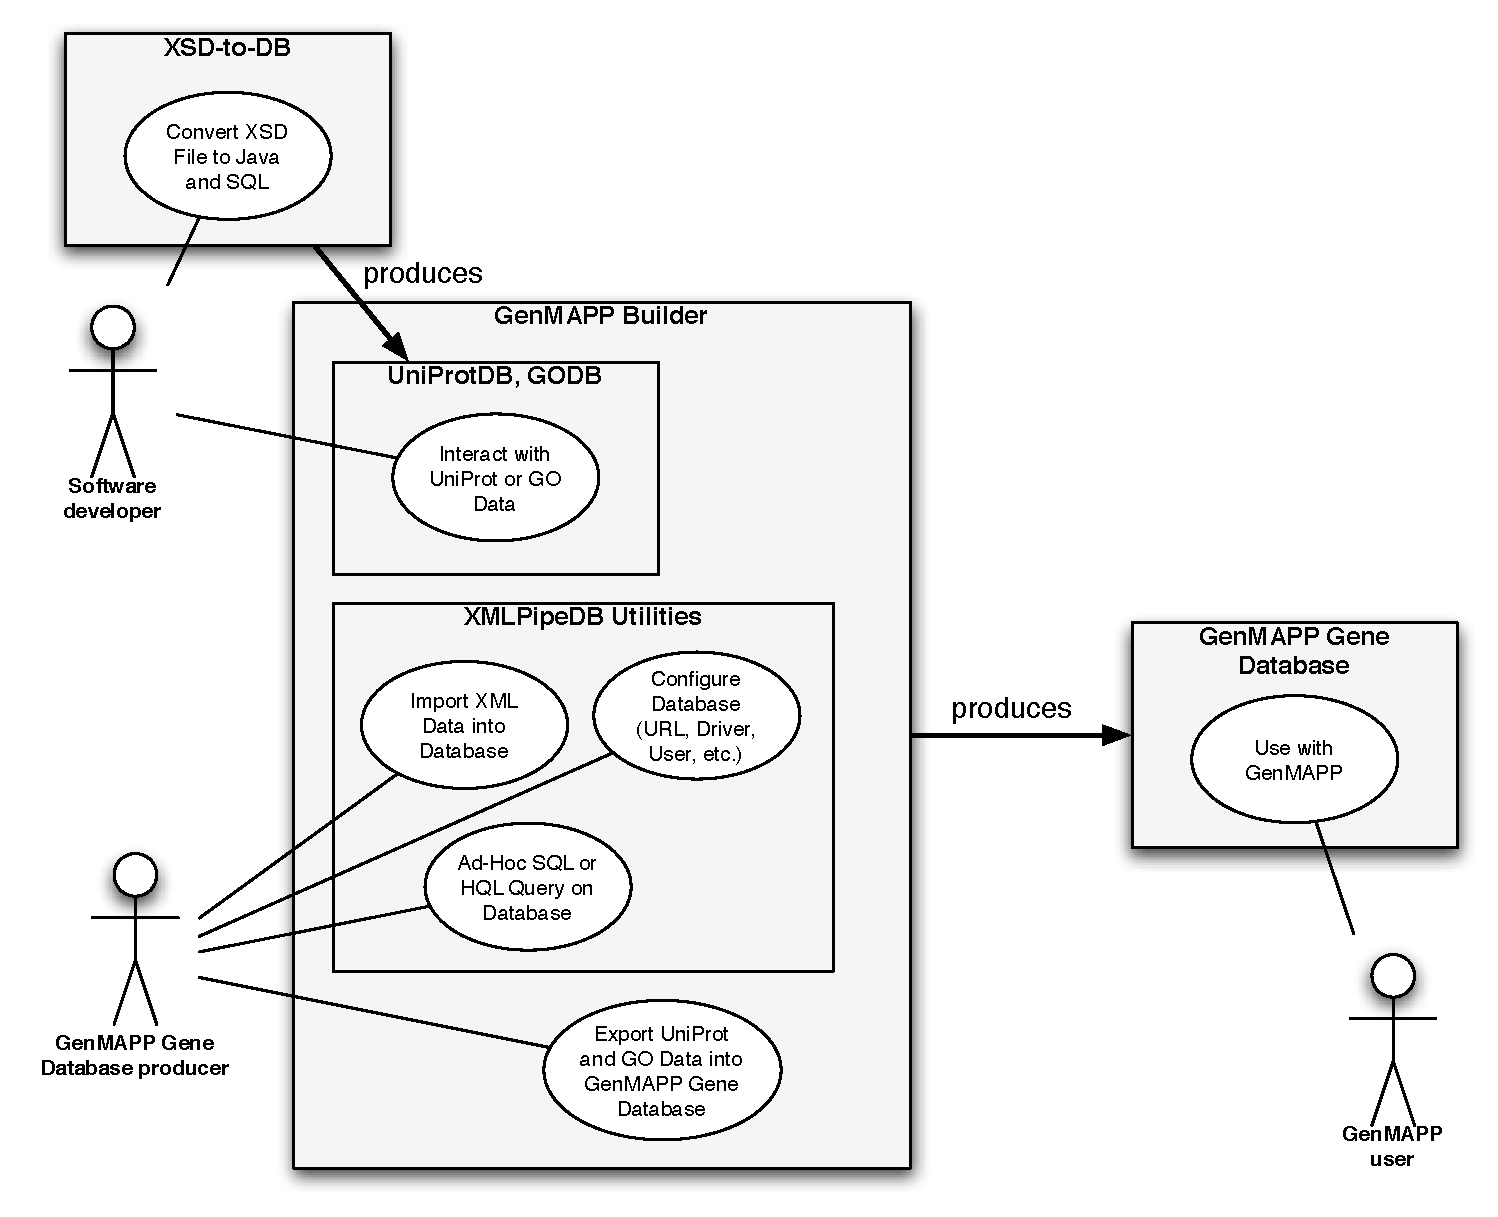
\includegraphics[width=5.5in]{figures/use-cases.pdf} 
   \caption{Use case model for the \xmlpipedb\ project.}
   \label{usecase}
\end{figure}

Need to explain the figure verbally\ldots\pb

\subsection*{\xsd2db}

The \xsd2db\ application takes a well-formed XML Schema (XSD) or Document Type Definition (DTD) file and converts it into a collection of Java source code and Hibernate mapping files that allows XML files based on that XSD or DTD to be read into a relational database.  It was used to help create the UniProtDB and GODB libraries which are used by GenMAPP Builder.\pb

\xsd2db's conversion functions are based on the open-source Hyperjaxb2 project (\url{https://hyperjaxb2.dev.java.net}).  It requires the following information to do its work:
\begin{itemize}
\item URL for the XSD or DTD file to process; in the case of a locally-loaded XSD or DTD, a \url{file:///} URL may be used

\item Hyperjaxb2 binding file

\item Directory that will contain its output
\end{itemize}
\xsd2db\ comes with a default binding file, which it copies into its output directory when it is invoked for the first time.  Additional customization can then be performed on the copied binding file, and subsequent invocations of \xsd2db\ will use that binding instead of the default.\pb

\xsd2db's primary requirement is the URL of the XSD or DTD file to convert.  \xsd2db\  processes this URL to produce Java source code, Hibernate mapping files, and an SQL DDL file that corresponds to the schema defined by the XSD file.\pb

\xsd2db\ behaves a little differently depending on the presence of certain files in the output directory, or even the presence of the output directory itself.  If the output directory is not present, then \xsd2db\ does the following:
\begin{enumerate}
\item Create the output directory.
\item Copy the XSD file from its given URL to the output directory.
\item Copy the default \xsd2db\ bindings file to the output directory.
\end{enumerate}
If the output directory already exists, then \xsd2db\ looks for the XSD and bindings files at the expected locations within that directory.  If those files are not present, then it performs the same steps as before.
\begin{itemize}
\item \xsd2db\ can be told whether or not to update the XSD file from its URL, in case the XSD file might have changed.  If it is told to perform an update, it will ask for the URL of the updated XSD file.
\end{itemize}
Once the output directory has been set up, \xsd2db\ then processes the XSD and bindings files to generate:
\begin{itemize}
\item Java source code for classes represented in the XSD
\item SQL DDL file defining the relational database tables that correspond to the Java classes
\item Hibernate mapping files that determine how the Java classes are convert to and from the relational tables
\item An Apache Ant \texttt{build.xml} file which can compile everything into a Java archive, ready for further development or deployment
\end{itemize}
From this point, a typical workflow would be:
\begin{enumerate}
\item Build a relational database using the generated SQL DDL file
\item Build the database library using the supplied Ant file, then use that library to test XML import, queries, and other database functions
\item Edit the bindings file to customize, correct, or improve the Java classes, Hibernate mappings, and relational tables generated from the XSD file
\item Re-run \xsd2db\ to actually create the new files
\end{enumerate}
Certain conversions might not be adequate even with extensive editing of the bindings file; in this case, the last resort is to manually edit the Java, Hibernate, and SQL files generated by \xsd2db\.  If this is done, be careful about re-running \xsd2db\ on this particular output directory --- \xsd2db\ \emph{always} generates the Java, Hibernate, and SQL files ``from scratch,'' using the XSD and bindings files in the output directory.\pb

Typically, once the generated files work as desired, the output directory becomes a software project in and of itself, to be edited, debugged, tested, and deployed like any other database library.  The fact that it was initially generated by \xsd2db\ merely indicates that some time was saved in creating this database library as compared to a manual Java-to-relational implementation of the XSD file.\pb

\xsd2db\'s output directory structure is shown in Figure~\ref{output}.  Directories are shown in boldface, and files are shown in italics.  Names in parentheses indicate placeholders for specific names that depend on the XSD being converted.\pb

\begin{figure}[htbp] %  figure placement: here, top, bottom, or page
   \centering
   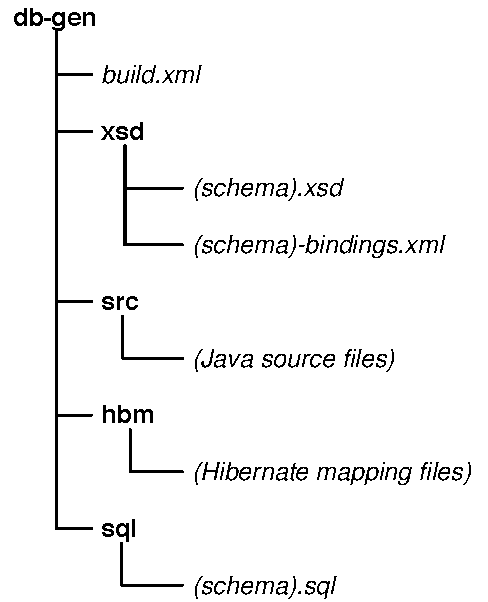
\includegraphics[width=2in]{figures/db-gen.pdf} 
   \caption{Structure of an \xsd2db\ output directory.}
   \label{output}
\end{figure}

The actual filenames and contents of terms in angle brackets $(< >)$ depend on the XSD file that was used to generate the output.  For instance, the UniProtDB library has \texttt{uniprot.xsd}, \texttt{uniprot-bindings.xml}, and \texttt{uniprot.sql}.\pb

\subsection*{\xpdutils}

The \xpdutils\ library is a suite of Java classes that provide functions that are common to most \xmlpipedb\ database applications.  Specifically, the library includes reusable classes for:
\begin{itemize}
\item Loading of XML files into Java objects, and subsequent saving of these XML-derived Java objects to a relational database
\item Rudimentary query and retrieval of Java objects from the relational database
\item Configuring a client application to communicate with a relational database
\end{itemize}
\xpdutils\ includes a sample GUI application that demonstrates these functions, using database code that was generated by \xsd2db.\pb

The \xpdutils\ library is separated into two layers: one layer provides the functionality, meant to be called programmatically, and another layer is a set of user interface components that allow end-user to invoke those functions.  The \xpdutils\ library relies heavily on JAXB and Hibernate --- in many respects, it is a convenience and GUI layer for these packages --- so knowledge of these APIs is very helpful in making full use of \xpdutils.\pb

\subsubsection*{Utility Functions}

The following classes implement the functions provided by \xpdutils:
\begin{itemize}
\item \texttt{ImportEngine} provides a \emph{loadToDB()} method, which takes any compliant input stream, parses it into its corresponding objects, then commits the objects to the database.

\item \texttt{ConfigurationEngine} is the centralized location for configuration information used by XMLPipeDB.  It provides functions for retrieving, setting, and validating configuration properties. The ConfigurationEngine also has a method for obtaining a Hibernate Configuration object, which is needed by ImportEngine and QueryEngine. The configuration object, however, only contains the Hibernate properties and NOT the mapping files. Hibernate mappings must be added by the caller before passing the Configuration object to the Query or Import Engines.

\item \texttt{QueryEngine} is a generalized query wrapper whose \emph{executeHQL()} function takes a Hibernate query (in HQL, Hibernate Query Language) and returns the results as a Java iterator.
\end{itemize}
Programs using the \xpdutils\ library can invoke these functions as necessary, using whatever mechanism is most appropriate for a particular application.\pb

\subsubsection*{User Interface Components}

To ease the development and delivery of these functions to end-user applications, \xpdutils\ also includes a component library that can be added directly into Java Swing windows and panels.  Each component provides a ``hook function'' that invokes the underlying operation, assuming that sufficient information has been gathered by the component:
\begin{itemize}
\item \texttt{ImportPanel} provides a front end for database imports, displaying components like file choosers, text editors, and preview panels to make database loading as easy as possible for end-users.

\item \texttt{ConfigurationPanel} provides a front-end for the properties in \texttt{ConfigurationEngine}.  The components are designed to be easily added to dialog boxes or preferences windows, and provide direct hooks to the \texttt{Configurator} functions.

\item \texttt{HQLPanel} allows users to enter an HQL (Hibernate Query Language) or SQL (Structured Query Language) query then provides a table or object browser that displays the results of that query.  This is meant primarily for debugging or advanced purposes, as it requires knowledge of the underlying database schema and/or domain object model.  HQL queries are processed by \texttt{QueryEngine}.
\end{itemize}
The demo application that comes with \xpdutils\ shows how these components are used, and how they interact with the underlying functionality.  GenMAPP Builder also uses \xpdutils\ for its import, configuration, and query functions.\pb

\subsection*{Database Libraries}

\xmlpipedb\ has used \xsd2db\ to generate Java database libraries for UniProt and Gene Ontology (GO) data sources, called UniProtDB and GODB, respectively.  These database libraries use JAXB to convert XML files from these data sources into Java objects, then use Hibernate to persist these Java objects in a relational database, a schema for which is provided with the distribution.\pb

The libraries work like standard JAXB applications when importing XML files: the data in the loaded file gets converted into a set of corresponding objects.  The libraries then work like standard Hibernate applications when saving these objects to the database: configure Hibernate, then use its classes to save/update the objects or to perform HQL queries.\pb

\subsubsection*{UniProtDB}

UniProtDB is the library of Java classes that allows UniProt XML files to be transferred into a relational database.  GenMAPP Builder uses the UniProtDB library; in turn, the UniProtDB library is semi-automatically generated from the \xmlpipedb\ project's \xsd2db\ tool.\pb

\xsd2db's ``as is'' output from reading the UniProt XSD \cite{uniprotxsd} required some post-processing prior to becoming usable in database applications.  Specifically, the following changes needed to be made:
\begin{itemize}
\item The UniProt XSD defines an \textsl{end} element.  Unfortunately, \textsl{end} is an SQL reserved word.  Thus, the post-processor renames \textsl{end} to \textsl{endPosition}.

\item Some XSD data types, particularly the range of options for XML dates, are not easily supported in SQL.  In particular, XSD dates allow month-year values with unspecified dates, or even just years.  This does not translate well to SQL and Java.  It was concluded that values which were defined this way in the UniProt XSD can acceptably be represented as strings.  This date mismatch occurred only once, in UniProt's \textsl{citationType} definition.  \textsl{citationType}'s \textsl{date} attribute was defined as:

\begin{verbatim}
<xs:simpleType>
    <xs:union memberTypes="xs:date xs:gYearMonth xs:gYear"/>
</xs:simpleType>
\end{verbatim}

\item Another data type issue concerns strings.  The libraries used by XSD-to-DB translated strings into SQL \texttt{varchar(255)}.  However, many string values in UniProt XML files exceed 255 characters in length.  Thus, instances of \texttt{varchar(255)} are converted into just \texttt{varchar} (unspecified length).
\end{itemize}
The UniProtDB post-processor is included in the \texttt{tools} subdirectory of the \texttt{uniprotdb} module in the \xmlpipedb\ repository.  Note that the post-processor only needs to be invoked if the UniProtDB files have been rewritten by \xsd2db.  As committed and released, the files in the repository are already post-processed.\pb

\subsubsection*{GODB}

Information from the GO (Gene Ontology) database is required to run GenMAPP Builder.  GODB provides a library of Java classes and Hibernate mapping (HBM) files that allows data from GO OBO XML files to be transfered into a relational database.\pb

XSD-to-DB's ``as is'' output from reading the GO DTD \cite{godtd} required some post-processing prior to becoming usable in database applications.  Specifically, the following changes needed to be made:
\begin{itemize}
\item The GO DTD defines an \textsl{to} element.  Unfortunately, \textsl{to} is an SQL reserved word.  Thus, the post-processor renames \textsl{to} to \textsl{to\_}.

\item Another data type issue concerns strings.  The libraries used by XSD-to-DB translated strings into SQL \texttt{varchar(255)}.  However, many string values in GO OBO XML files exceed 255 characters in length.  Thus, instances of \texttt{varchar(255)} are converted into just \texttt{varchar} (unspecified length).
\end{itemize}
The GODB post-processor is included in the \texttt{tools} subdirectory of the \texttt{godb} module in the \xmlpipedb\ repository.  Note that the post-processor only needs to be invoked if the GODB files have been rewritten by \xsd2db.  As committed and released, the files in the repository are already post-processed.\pb

GODB needs to be regenerated if the GO OBO XML DTD changes.  However, in this case, the utility provide to do the post processing, \texttt{GodbPostProcessor}, may also need to be updated, since new issues may be introduced with the GO schema change.\pb

\subsubsection*{Database Administration and Setup}

The applications and libraries in \xmlpipedb\ require any relational database for which a JDBC driver exists.  Thus, they all require some degree of configuration, for specifying the database server, database name, username, password, etc.  To facilitate this, \xpdutils\ includes a common database configuration GUI in all of its applications.  Any other mechanism may also be used if desired, since database access is strictly ``standard'' JDBC and/or Hibernate.\pb

\subsection*{End-User Software}
\label{endUserSoftware}

\xsd2db, \xpdutils, UniProtDB, and GODB are primarily for software developers.  This section discusses the components of \xmlpipedb\ that are geared toward end-users, particularly bioinformaticians.\pb

\subsubsection*{Pre-Built GenMAPP Gene Database Files}
\label{gdb}

For users whose primary interest is to run GenMAPP for a particular organism, the \xmlpipedb\ group has used \gmb\ to produce the following GenMAPP gene database files from UniProt XML sources.  They were constructed for direct use by GenMAPP; once GenMAPP has been ``pointed'' to these files, they can be used immediately with expression data sets for their respective organisms:
\begin{itemize}
\item \ecolifull\ K12
\item \athalianafull
%\item \species{Pseudomonas putida}
%\item \species{Bacillus subtilis}
\end{itemize}

GenMAPP (Gene Map Annotator and Pathway Profiler) is a free computer application for 
viewing and analyzing DNA microarray and other genomic and proteomic data on biological pathways.   MAPPFinder is an accessory program that works with GenMAPP and Gene Ontology to identify global biological trends in gene expression data. The GenMAPP Gene Database (file with the extension \texttt{.gdb}) is used to relate gene IDs on MAPPs (\texttt{.mapp}, representations of pathways and other functional groupings of genes) to data in Expression Datasets (\texttt{.gex}, DNA microarray or other high-throughput data).  GenMAPP is a stand-alone application that requires the Gene Database, MAPPs, and Expression Dataset files to be 
stored on the user's computer. GenMAPP and its accessory programs and files may be downloaded from \url{http://www.GenMAPP.org}.  GenMAPP requires a separate Gene Database for each species.\pb






%%%%%%%%%%%%%%%%%%%%%%%%%%%%
%% Results and Discussion %%
%%
\section*{Results and Discussion}

\subsection*{Functionality}

Does the software do what we want it to do?\pb

\subsection*{Extensibility}

What range of XSD and DTD schemas does the software support?  (mention the issue encountered with MAGE-ML)\pb

How easily does \gmb\ export new species?  (most of Jeffrey's work would live here?)\pb

\subsection*{Performance}

Size vs.\ speed differences between \ecoli\ and \athaliana\ imports/exports.\pb
    

%%%%%%%%%%%%%%%%%%%%%%
\section*{Conclusions}
  Text for this section \ldots



%%%%%%%%%%%%%%%%%%%%%%%%%%%%%%%%%%%%%%%%
\section*{Availability and Requirements}

\begin{description}
\item[Project name:] XMLPipeDB
\item[Project home page:] \url{http://xmlpipedb.cs.lmu.edu}
\item[Operating system(s):] Libraries are platform-independent; GenMAPP Builder requires a Microsoft Windows operating system with a compatible version of the Jet (Access) database engine
\item[Programming language:] Java
\item[Other requirements:] Relational database management system for which a Java Database Connectivity (JDBC) driver is available; authors have been using PostgreSQL
\item[License:] LGPL
\item[Any restrictions to use by non-academics:] TBD
\end{description}


%%%%%%%%%%%%%%%%%%
\section*{List of Abbreviations}

% Optional, according to instructions; if not included, abbreviations
% must be explained in the text.

\begin{description}
\item[JDBC]
\item[ORM]
\item[XML]
\end{description}

    
%%%%%%%%%%%%%%%%%%%%%%%%%%%%%%%%
\section*{Authors' contributions}

% Per suggested format in instructions.

KDD did \ldots  JN did \ldots  JDD did \ldots  All authors read and approved the final manuscript.

    

%%%%%%%%%%%%%%%%%%%%%%%%%%%
\section*{Acknowledgements}
  \ifthenelse{\boolean{publ}}{\small}{}

  Text for this section \ldots


 
%%%%%%%%%%%%%%%%%%%%%%%%%%%%%%%%%%%%%%%%%%%%%%%%%%%%%%%%%%%%%
%%                  The Bibliography                       %%
%%                                                         %%              
%%  Bmc_article.bst  will be used to                       %%
%%  create a .BBL file for submission, which includes      %%
%%  XML structured for BMC.                                %%
%%                                                         %%
%%                                                         %%
%%  Note that the displayed Bibliography will not          %% 
%%  necessarily be rendered by Latex exactly as specified  %%
%%  in the online Instructions for Authors.                %% 
%%                                                         %%
%%%%%%%%%%%%%%%%%%%%%%%%%%%%%%%%%%%%%%%%%%%%%%%%%%%%%%%%%%%%%


{\ifthenelse{\boolean{publ}}{\footnotesize}{\small}
 \bibliographystyle{bmc_article}  % Style BST file
  \bibliography{xmlpipedb-refs} }     % Bibliography file (usually '*.bib' ) 

%%%%%%%%%%%

\ifthenelse{\boolean{publ}}{\end{multicols}}{}

%%%%%%%%%%%%%%%%%%%%%%%%%%%%%%%%%%%
%%                               %%
%% Figures                       %%
%%                               %%
%% NB: this is for captions and  %%
%% Titles. All graphics must be  %%
%% submitted separately and NOT  %%
%% included in the Tex document  %%
%%                               %%
%%%%%%%%%%%%%%%%%%%%%%%%%%%%%%%%%%%

%%
%% Do not use \listoffigures as most will included as separate files

\section*{Figures}
  \subsection*{Figure 1 - Sample figure title}
      A short description of the figure content
      should go here.

  \subsection*{Figure 2 - Sample figure title}
      Figure legend text.



%%%%%%%%%%%%%%%%%%%%%%%%%%%%%%%%%%%
%%                               %%
%% Tables                        %%
%%                               %%
%%%%%%%%%%%%%%%%%%%%%%%%%%%%%%%%%%%

%% Use of \listoftables is discouraged.
%%
\section*{Tables}
  \subsection*{Table 1 - Sample table title}
    Here is an example of a \emph{small} table in \LaTeX\ using  
    \verb|\tabular{...}|. This is where the description of the table 
    should go. \par \mbox{}
    \par
    \mbox{
      \begin{tabular}{|c|c|c|}
        \hline \multicolumn{3}{|c|}{My Table}\\ \hline
        A1 & B2  & C3 \\ \hline
        A2 & ... & .. \\ \hline
        A3 & ..  & .  \\ \hline
      \end{tabular}
      }
  \subsection*{Table 2 - Sample table title}
    Large tables are attached as separate files but should
    still be described here.



%%%%%%%%%%%%%%%%%%%%%%%%%%%%%%%%%%%
%%                               %%
%% Additional Files              %%
%%                               %%
%%%%%%%%%%%%%%%%%%%%%%%%%%%%%%%%%%%

\section*{Additional Files}
  \subsection*{Additional file 1 --- Sample additional file title}
    Additional file descriptions text (including details of how to
    view the file, if it is in a non-standard format or the file extension).  This might
    refer to a multi-page table or a figure.

  \subsection*{Additional file 2 --- Sample additional file title}
    Additional file descriptions text.


\end{bmcformat}
\end{document}







